%----------------------------------------------------------------------------------------
%	PACKAGES AND OTHER DOCUMENT CONFIGURATIONS
%----------------------------------------------------------------------------------------

\documentclass[final,hyperref={pdfpagelabels=false}]{beamer}

\usepackage[orientation=portrait,size=a0,scale=1.15,22pt]{beamerposter} % Use the beamerposter package for laying out the poster with a portrait orientation and an a0 paper size

%\usepackage{fontenc}

\usepackage{units}
\usepackage{siunitx}
\usepackage{graphicx}
\usepackage{graphicx, caption, subcaption}
\usepackage{geometry,array,graphicx,float,caption}
\usepackage{subcaption}
\usepackage[version=3]{mhchem} % Formula subscripts using \ce{}
\usepackage{physics}

%\usepackage{fontspec}
%\setsansfont{Futura LT Pro}
%\renewcommand{\bfseries}{\relax}

%\usepackage[sfdefault,lining]{FiraSans} %% option 'sfdefault' activates Fira Sans as the default text font
%\usepackage[fakebold]{firamath-otf}
%\renewcommand*\oldstylenums[1]{{\firaoldstyle #1}}
%\usepackage[T1]{fontenc}
%\usepackage[sfdefault,scaled=1]{FiraSans}
%\usepackage{newtxsf}
%\usepackage{arev}

\usepackage[T1]{fontenc}
\usepackage[sfdefault]{FiraSans}
\usepackage{newtxsf}

\newcommand{\cref}{c^{\ominus}}
\newcommand{\Hplus}{\text{H}^{+}}
\newcommand{\Aminus}{\text{A}^{-}}


%\usepackage[italic]{mathastext}
% 'isomath' sets upper case greek letters italic in accordance with 
% the International Standard ISO 80000-2
%\usepackage{isomath}

\usetheme{I6pd2} % Use the I6pd2 theme supplied with this template
\usepackage[english]{babel} % English language/hyphenation

\usepackage{amsmath,amsthm,amssymb,latexsym} % For including math equations, theorems, symbols, etc

\usepackage{subcaption}
%\captionsetup[subfigure]{list=true, font=large, labelfont=bf, labelformat=brace, position=top}


%\usepackage{times}\usefonttheme{professionalfonts}  % Uncomment to use Times as the main font
%\usefonttheme[onlymath]{serif} % Uncomment to use a Serif font within math environments

%\boldmath % Use bold for everything within the math environment

\usepackage{booktabs} % Top and bottom rules for tables

\graphicspath{{figures/}} % Location of the graphics files

\usecaptiontemplate{\structure{\insertcaptionname~\insertcaptionnumber: }\insertcaption} % A fix for figure numbering

%----------------------------------------------------------------------------------------
%	TITLE SECTION 
%----------------------------------------------------------------------------------------

\title{\textbf{\HUGE {\textcolor{dblue}{Path Integral}} Molecular Dynamics Simulations Using ESPResSo}\\\vspace{-5cm}\hspace{38.1cm}} % Poster title

%\title{\textbf{\VeryHuge Validity of NMR Relaxation\\ for the characterization of\\ coarse-grained models\\\vspace{-2.5cm}\hspace{38.1cm}} % Poster title

\author{\huge Devashish Tiwari,$^{1,2}$ David Beyer$^1$ \& Christian Holm$^1$} % Author(s)

\institute{$^1$Institute for Computational Physics, University of Stuttgart, Germany\\$^2$Indian Institute of Science Education and Research, Bhopal, India}

\usepackage{tikz}
\usetikzlibrary{tikzmark}
%\usetikzlibrary{shapes,snakes}

\setbeamertemplate{background canvas}{%
\begin{tikzpicture}[remember picture,overlay]
\shade[top color=white,bottom color=hblue, shading angle=0]
  ([shift={(0.0cm,0.0cm)}]current page.north west)
     rectangle
  ([shift={(0.0cm,0.0cm)}]current page.south east);
\end{tikzpicture}%     
}

\begin{document}

\addtobeamertemplate{block end}{}{\vspace*{2ex}} % White space under blocks

\begin{frame}[t] % The whole poster is enclosed in one beamer frame

\begin{columns}[t] 

\begin{column}{.48\textwidth} % The first column

\begin{block}{Motivation}
\begin{itemize}
\item Often important to consider quantum and thermal effects\\
\Rightarrow$ e.g. superfluids, quantum gases, isotope effects in crystals, etc.
\item Still may want to use more coarse-grained potentials rather than full electronic problem\\
$\Rightarrow$ Path integrals provide an elegant formalism
\end{itemize}
\end{block}

\begin{block}{Path Integrals in Quantum Statistics}
\textbf{Feynman path integral formalism} \cite{feynman48}:
\begin{itemize}
\item Transition amplitudes can be expressed as sum over paths:
\begin{align*}
\bra{x_bt_b}\ket{x_at_a} = \sum_{\text{all}\,\text{paths}\, x(t)} \exp\left(\frac{i}{\hbar}S[x(t)]\right)
\end{align*}
with action functional 
\begin{align*}
	S[x(t)] = \int_{t_a}^{t_b}\text{d}t\, L(x(t), \dot{x}(t), t)
\end{align*}
\item Follows from composition law of time evolution operator \cite{kleinert09}
\begin{align*}
\bra{x_bt_b}\ket{x_at_a} &= \bra{x_b}\exp\left(-\frac{i}{\hbar}(t_b-t_a)H\right)\ket{x_a} = \bra{x_b}U(t_b, t_a)\ket{x_a}\\
&= \bra{x_b}U(t_b,t_N)U(t_N,t_{N-1})\cdots U(t_1,t_a)\ket{x_a}
\end{align*}
and taking number of time slices $N\rightarrow\infty$:
\begin{align*}
\bra{x_bt_b}\ket{x_at_a} &= \int_{x(t_a)=x_a}^{x(t_b)=x_b} \mathcal{D} x(t) \exp\left(\frac{i}{\hbar}S[x(t)]\right)\\
	&\propto \lim_{N\rightarrow\infty} \prod_{n=1}^{N}\left[\int_{-\infty}^{\infty}\,\text{d}x_n\right] \exp\left(\frac{i}{\hbar}\mathcal{S}^N(x_1,...,x_N)\right)
\end{align*}
with time-sliced action $\mathcal{S}^N(x_1,...,x_N)$
\end{itemize}
\text{ }\\
\textbf{Wick rotation}:
\begin{itemize}
\item Analytical continuation to complex time:
\begin{align*}
t_b - t_a = -i\hbar \beta
\end{align*}
\item Transition amplitudes become matrix elements of density matrix:
\begin{align*}
\rho(x_a, x_b) = \bra{x_b}\exp\left(-\beta H\right)\ket{x_a} = \int_{x(0)=x_a}^{x(\tau = \hbar\beta)=x_b} \mathcal{D} x(\tau) \exp\left(-\frac{1}{\hbar}S_\text{e}[x(\tau)]\right)
\end{align*}
\item Partition function as path integral over closed paths:
\begin{align*}
Z = \text{Tr}\exp\left(-\beta H\right) = \int_{-\infty}^{\infty}\text{d} x\,\rho(x, x) = \oint \mathcal{D} x(\tau) \exp\left(-\frac{1}{\hbar}S_\text{e}[x(\tau)]\right)
\end{align*}
with "euclidean action" $S_\text{e}$\\
\text{}
\end{itemize}
\end{block}

\begin{block}{PIMD: Isomorphism with Classical Ring Polymers}
\begin{itemize}
\item Consider $1D$ quantum system with Hamiltonian
\begin{align*}
	H = \frac{p^2}{2m} + V(x)
\end{align*}
\item For finite $N$, partition function can be written as
\begin{align*}
Z \approx\text{const.}\times \prod_{n=1}^{N}\left[\int_{-\infty}^{\infty}\,\text{d}x_n\right] \exp\left(-\beta\left(\frac{\kappa}{2}\sum_{n=1}^N\left(x_n-x_{n+1}\right)^2+\frac{1}{N}\sum_{n=1}^NV(x_n)\right)\right)
\end{align*}
with PBC $x_{N+1}=x_1$\\
$\Rightarrow$ discretized euclidean action looks like Hamiltonian of classical ring polymer with harmonic bonds
\begin{align*}
V_{\text{bonded}}(x_n, x_{n+1})=\frac{\kappa}{2}\left(x_n-x_{n+1}\right)^2
\end{align*}
in external potential $V(x)$
\item \textbf{Path Integral Molecular Dynamics} (PIMD): use classical canonical MD to sample equilibrium distribution of ring polymer\\
$\Rightarrow$ here: use ESPResSo and Langevin dynamics
\end{itemize}

\begin{columns}[T,onlytextwidth]
\column{0.5\textwidth} 
\begin{figure}[H]
\centering
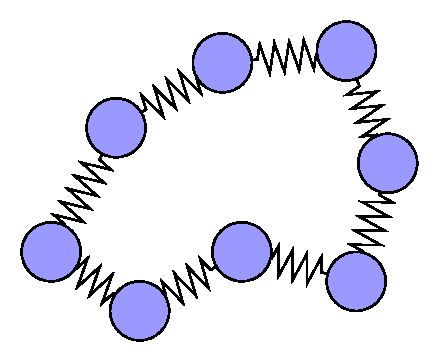
\includegraphics[width=0.7\textwidth]{figures/cg_schematic_neutral/cg_schematic_neutral.pdf}
\end{figure}

\column{0.5\textwidth} 
	\vspace{2cm}
\begin{figure}[H]
\centering
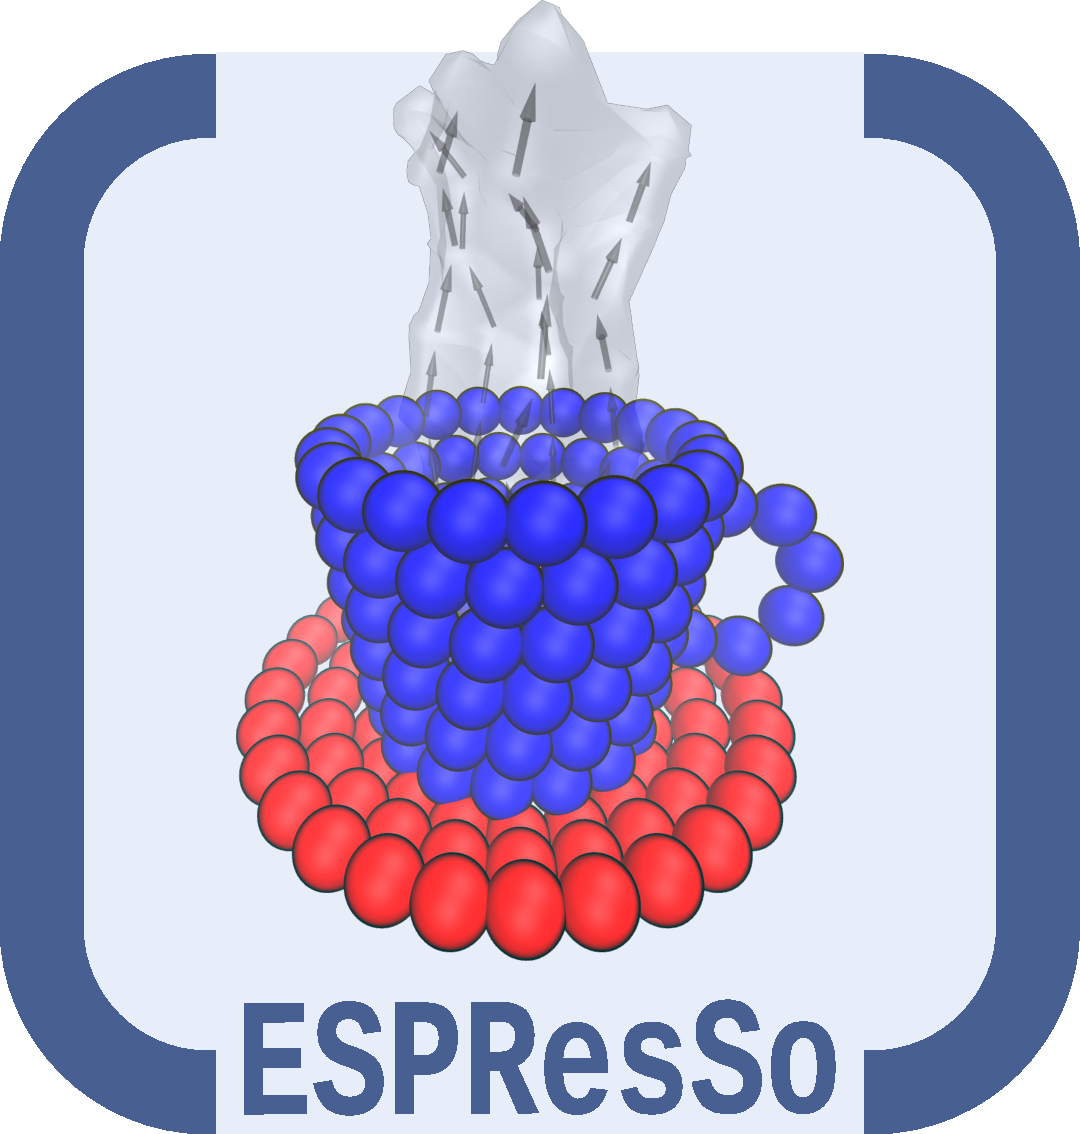
\includegraphics[width=0.4\textwidth]{figures/logo-espresso.pdf}
\end{figure}
\end{columns}
\end{block}

\end{column} % End of the first column


\begin{column}{.48\textwidth}

\begin{block}{Reaching the Continuum Limit}
\begin{itemize}
\item Model system -- 1D harmonic oscillator:
\begin{align*}
H = \frac{p^2}{2m} + \frac{m\omega^2x^2}{2}
\end{align*}
\item Mapping to classical ring polymers only exact in the limit $N\rightarrow \infty$\\
$\Rightarrow$ need to extrapolate by performing simulations for different $N$
\item Results for different lattice spacings $\delta\tau\propto 1/N$: 
\end{itemize}

\begin{figure}[H]
\centering
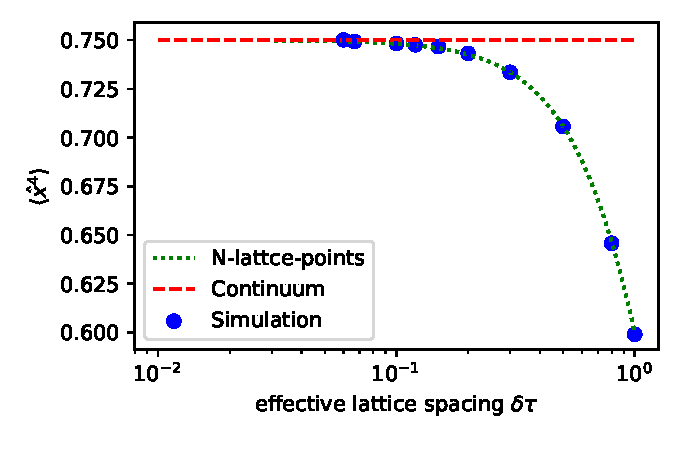
\includegraphics[width=0.5\textwidth]{figures/moments.pdf}
\end{figure}

\end{block}

\begin{block}{Density Matrix and Energy Levels}
\begin{itemize}
\item Diagonal $\rho(x,x)$ of density matrix can be directly obtained as histogram of monomer positions
\item Mean energy can be obtained using virial estimator:
\begin{align*}
U_{\text{v}}=\frac{1}{2N} \sum_{n=1}^N x_n V^{\prime}\left(x_n\right)+\frac{1}{N} \sum_{n=1}^N V\left(x_n\right)
\end{align*}
\end{itemize}

\begin{columns}[T,onlytextwidth]
\column{0.5\textwidth} 
\begin{figure}[H]
\centering
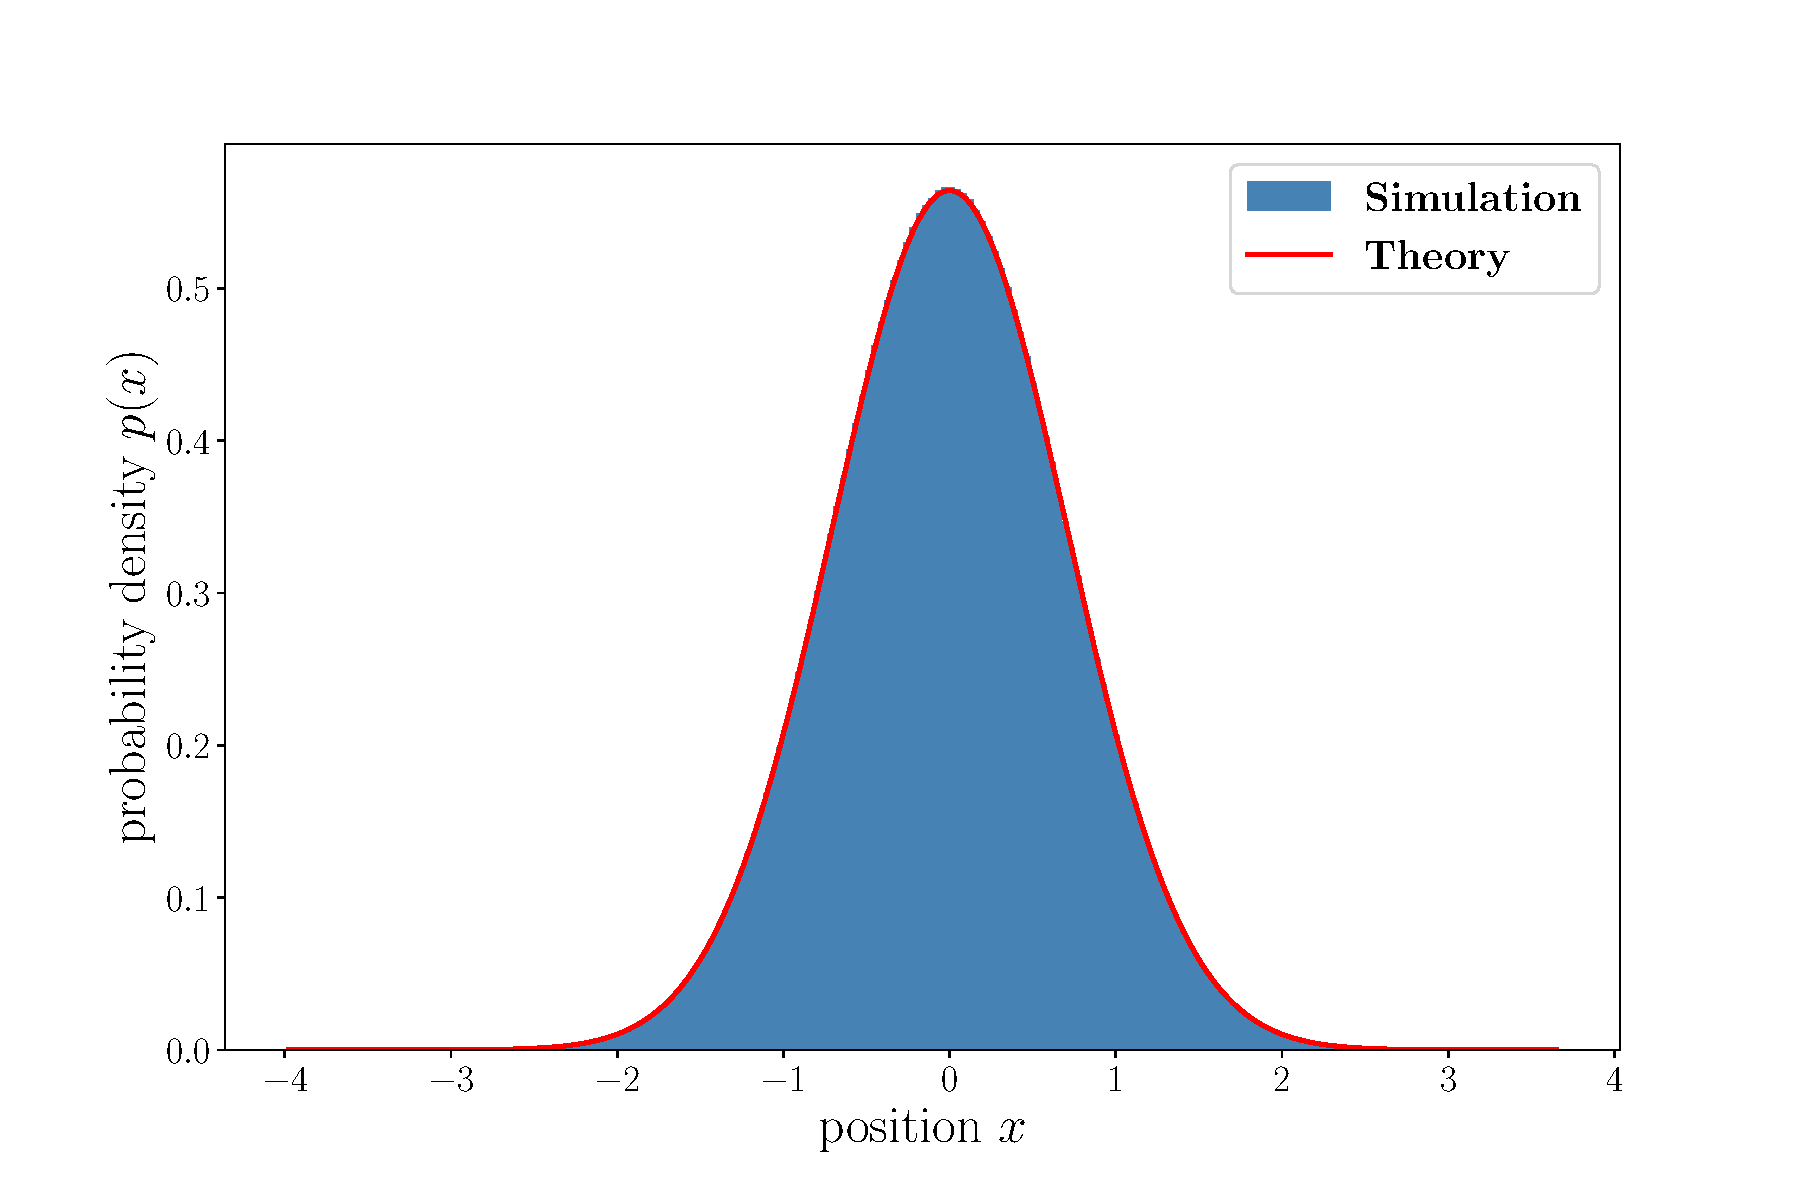
\includegraphics[width=\textwidth]{figures/density_matrix.pdf}
\end{figure}

\column{0.5\textwidth} 
\begin{figure}[H]
\centering
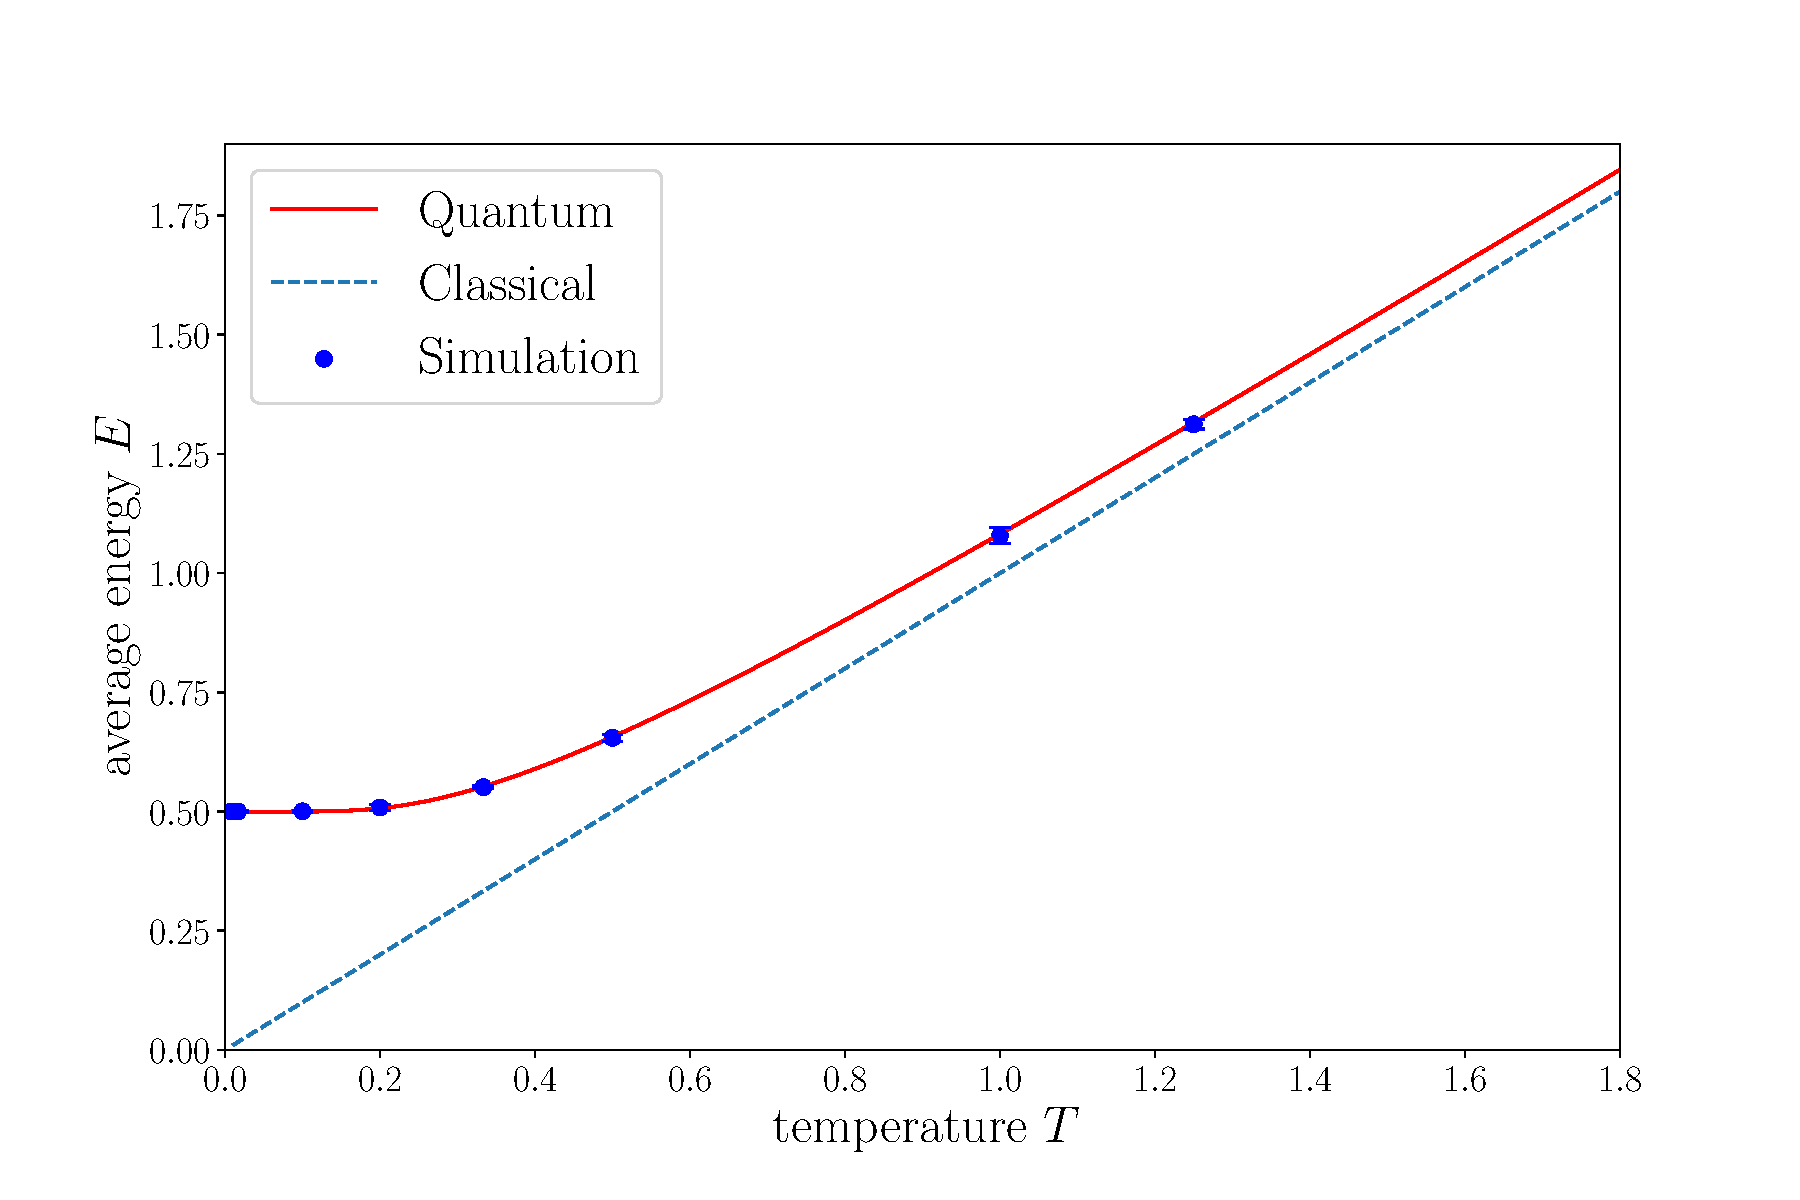
\includegraphics[width=\textwidth]{figures/energy.pdf}
\end{figure}
\end{columns}

\begin{itemize}
\item Energy-levels can be obtained using imaginary-time correlation functions, e.g.
\begin{align*}
\mathcal{A}(\Delta \tau) & =\langle \hat{x}(\tau) \hat{x}(\tau+\Delta \tau)\rangle = e^{-\left(E_1-E_0\right) \Delta \tau} \mathcal{A}(0)
\end{align*}
\end{itemize}

\begin{columns}[T,onlytextwidth]
\column{0.5\textwidth} 
\begin{figure}[H]
\centering
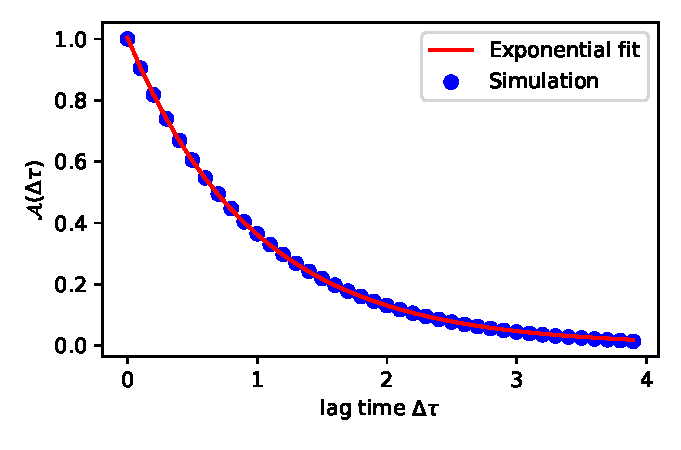
\includegraphics[width=\textwidth]{figures/two_point_correlation.pdf}
\end{figure}

\column{0.5\textwidth} 
	\vspace{3.5cm}
\begin{table}[ht]
    \centering
    \begin{tabular}{ccc} % Three columns, without vertical lines
        \toprule % Top horizontal rule
        & $E_n - E_0$ & Error \\
        \midrule % Middle horizontal rule
        2 point & 1.01947 & 0.04 \\
        4 point & 2.00502 & 0.07 \\
        \bottomrule % Bottom horizontal rule
    \end{tabular}
\end{table}

\end{columns}

\end{block}

\begin{block}{Conclusion and Outlook}
\begin{itemize}
\item PIMD in ESPResSo allows to reproduce analytical results for quantum harmonic oscillator
\item Next step: include permutation moves to correctly model Bose-Einstein statistics in many-body systems
\end{itemize}
\end{block}

\vspace{-0.05cm}
\begin{block}{References}
\begin{thebibliography}{9}
{
\bibitem{feynman48}
\textsc{Richard Feynman},
\emph{Space-Time Approach to Non-Relativistic Quantum Mechanics}, 
Rev. Mod. Phys.,
vol. 20,
1948.
}
{
\bibitem{kleinert09}
\textsc{Hagen Kleinert},
\emph{Path Integrals in Quantum Mechanics, Statistics, Polymer Physics, and Financial Markets}, 
World Scientific,
2009.
}
{
\bibitem{ceperley}
\textsc{David Ceperley},
\emph{Path integrals in the theory of condensed helium}, 
Rev. Mod. Phys.,
vol. 67,
1995.
}
{
\bibitem{westbroek}
\textsc{Marise Westbroek} et al.,
\emph{User's guide to Monte Carlo methods for evaluating path integrals}, 
Am. J. Phys.,
vol. 86,
2018.
}
\end{thebibliography}
\end{block}



\end{column}

\end{columns}

%----------------------------------------------------------------------------------------



\end{frame} % End of the enclosing frame

\end{document}
